\ofsubsection{Chocobo}
%

\ofquote{"There's no wrong way to love a chocobo."\\}{Noctis}\\\\
%
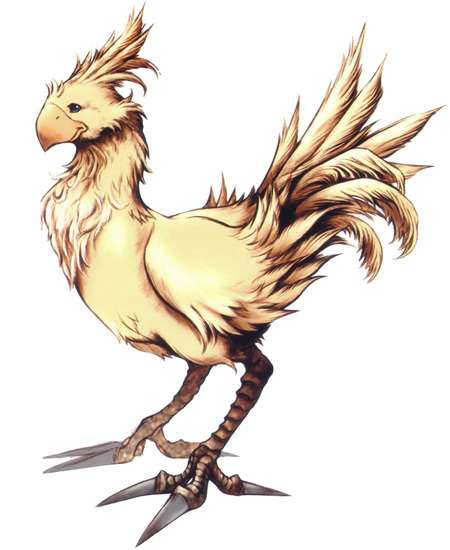
\includegraphics[width=0.95\columnwidth]{./art/chocobo/chocobo.jpg}
%
\\\\
%
%
\accf{Chocobos} are large, flightless avian creatures with yellow feathers and a long neck.
They are very intelligent and even understand humanoid languages to some degree.
Therefore, Chocobos are often domesticated and used as mounts, making them comparable to horses and renting out Chocobos is a lucrative business for farmers.
Although prices may fluctuate, the party can usually rent a Chocobo for about 10G per day.
In rare cases, farmers also sell Chocobo at extremely expensive prices, starting at around 3000G. 
Alternatively, the party can try to catch Chocobos that roam in the wild, they can usually be found in forests or wide grasslands.
Such Chocobos generally consider them to be hostile by default and engage in combat when feeling threatened.
When taking any damage, a wild Chocobo performs a DC~7 check and upon failure it becomes scared and flees as quickly as possible.
A character can gain its trust by using their action to feed it a Chocobo's favorite food, the \accf{Gysahl Greens}.
In this case, the player performs a check with a DC of 6 + the Chocobo's Level and if successful, it will join the party and follow his or her command from now on.
%
\ofpar
%
%\ofquote{"Fat Chocobo? You're rude! Here it's the bird of gods!"}{Dwarf}\\\\
%
As most avian creatures, Chocobos lay eggs from which their babies hatch.
However, they grow surprisingly quickly: an egg hatches a few weeks after it is laid and after another month, 
most Chocobos are already as large as their owner.  
They are usually bred in stables, where they can be kept in a warm and safe environment.
Chocobos can be of different types, which is determined by the color of their feathers.
The most common one is the yellow Chocobo, other types are rather rare compared to it.
A Chocobo's type depends on its parents and the following table shows the outcome of different pairings.
In all cases that are not listed, a Chocobo has its parents' type if they are both the same and it is yellow otherwise.\\\\
%
\oftable{p{0.37\columnwidth} p{0.37\columnwidth} p{0.3\columnwidth}}
{\accf{Parent 1} & \accf{Parent 2} & \accf{Child}} {
Yellow 	& Blue   & Green \\
Yellow 	& Red    & Green \\
Blue 	& Green  & Red \\
Red 	& Green  & Blue \\
Blue 	& Blue   & White \\
Red 	& Red    & Black \\
Black 	& White  & Gold\\
}
%
\vfill
%
This knowledge is available at many experienced Chocobo breeders or in books about the topic.
The party can try to breed some of the rare types, which often come with special abilities.
Details about the different Chocobo types are shown at the end of this subsection.
In some cases a newly born Chocobo's type might not adhere to the table above.
Whenever a new Chocobo is born, make a DC 11 check and if you succeed, its type is instead determined as follows:
roll 2d, the Chocobo is white on 2-3, blue on 4-5, yellow on 6-8, red on 9-10, black on 11-12.
%
%\ofpar
%
Raising a Chocobo is not a simple task, as they require a lot of care and attention.
In return, a Chocobo can the help the party in various ways through their unique capabilities, which improve throughout the adventure.
As such, the current experience of a Chocobo is tracked through its Level, the same way as for player characters. 
However, Level ups are performed slightly differently for Chocobos.
Firstly, a Chocobo can only learn a pre-determined set of abilities depending on its type.
Secondly, the attribute increases at Level up are also handled differently for Chocobos:
their maximum HP and MP increase both by 5 at each Level up. 
In addition, its owner can spend an additional 3 points to further improve the Chocobo's attributes as desired.
The table below shows how many points need to be spent for different attribute bonuses.
A final noteworthy difference compared to player characters is that Chocobos posses the additional \accf{Stamina~(STA)} attribute, which determines their affinity for long distance travel.
%
\ofpar
%
\oftable{p{0.5\columnwidth} p{0.3\columnwidth}} 
{\accf{Attribute Bonus} & \accf{Required Points}} {
  Max. HP +5 	& 1 \ofrow
  Max. MP +5 	& 1 \ofrow
  STR +1 		& 1 \ofrow
  DEF +1 		& 1 \ofrow
  MAG +1 		& 1 \ofrow
  RES +1 		& 1 \ofrow
  STA +1 		& 2 \ofrow
  DMG +1d 		& 3 \ofrow
  AGI +1 		& 3 \ofrow
}
%
\clearpage
%
%\ofquote{"Man... Chocobo, we just can’t get a break, can we?"\\}{Sazh}\\\\
\ofquote{"My hair does NOT look like a Chocobo's butt!"\\}{Prompto}\\\\
%
Characters can ride Chocobos for a fast and comfortable travel experience.
Riding domesticated ones is simple, but a more experienced rider may come out ahead in sticky situations.
They can carry a reasonable amount of weight without being affected.
Nevertheless, Chocobos get tired after too much uninterrupted travel time.
A Chocobo can walk an amount of hours equal to its Stamina attribute before it needs a break.
This time is halved, if the carried total weight significantly exceeds that of two average humans.
Even though Chocobos usually follow their owner's orders, they might refuse to keep going whenever they are particularly scared or caught by surprise.
Chocobos can also be very capable combatants and thus crucial additions to the party line-up.
They can fight alongside the party, in which case they are treated as any other allied combat participant.
A Chocobo is controlled by the player whose character is its owner and it obeys their commands.
Alternatively, characters can also decide to stay mounted on their Chocobo during combat.
If they do so, the Chocobo and its owner always take their turn together, where only the Chocobo handles the movement. 
Whenever the rider Attacks a small or medium sized enemy while mounted, the target has Disadvantage on the evasion check.
However, when the Chocobo suffers damage while carrying a rider, it has to make a check with a DC of 12 minus its STR attribute. 
If it fails this check, the rider is thrown off and suffers Immobile for 1 round.
%
\vfill
%
\ofmonster{Yellow Chocobo}{1}{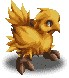
\includegraphics[width=0.23\columnwidth]{./art/chocobo/chocyellow.jpg}}
{
	HP: & \hfill 19 & MP: & \hfill 17\\
	STR: & \hfill 1 & DEF: & \hfill 0 \\
	MAG: & \hfill 1 & RES: & \hfill 0 \\
	AGI: & \hfill 2 & STA: & \hfill 2 \\
}
{\accf{Beak}: 1d DMG}
{
	\mspell{Cure (Level 1)}{4}{0r}{Single}{3u}{The target regains 2d HP.}{\accf{Level 1}}		
	\mspell{Esuna (Level 3)}{6}{0r}{Single}{5u}{Remove all Status Effects except KO.}{\accf{Level 3}}	
	\mtech{Enrage (Level 6)}{10}{0r}{Single}{5u}{The target performs a DC 8 check and upon failure he has to move towards you on his next turn and if possible perform an Attack on you.}{\accf{Level 6}}	
	\mtech{Fat Chocobo (Level 9)}{16}{1r}{1u}{5u}{Everyone in the target area suffer 6d damage and Immobile for 1 round.}{\accf{Level 9}\immobile}	
	\mpassive{Choco Glide}{You can glide down slowly from heights up to 30u without taking any damage.}
}
%
\newpage
%
\ofquote{"Ya know, all I want to do is ride on a chocobo. Faster than the wind!"}{Clasko}\vfill
%
\ofmonster{Red Chocobo}{1}{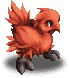
\includegraphics[width=0.23\columnwidth]{./art/chocobo/chocred.jpg}}
{
	HP: & \hfill 21 & MP: & \hfill 13\\
	STR: & \hfill 2 & DEF: & \hfill 1 \\
	MAG: & \hfill 0 & RES: & \hfill 0 \\
	AGI: & \hfill 2 & STA: & \hfill 2 \\
}
{\accf{Beak}: 1d DMG \hfill \accf{Resilient:}\fire}
{	
	\mtech{Choco Kick (Level 1)}{4}{0r}{Single}{Weapon}{The target suffers 2d damage and is knocked back by 1u.}{\accf{Level 3}}
	\mtech{Choco Dash (Level 3)}{7}{0r}{5u (line)}{Self}{You dash in a line of up to 5u dealing 3d damage to everyone in the target area and knocking them to the side by 1u.}{\accf{Level 6}}
	\mtech{Choco Blaze (Level 6)}{14}{0r}{3u}{Self}{Everyone in the target area except you suffers 5d fire damage.}{\accf{Level 9}\fire}
	\mreaction{Choco Counter}{Whenever you are hit by an Attack, immediately make an Attack on the perpetrator.}
	\mpassive{Choco Jump}{You can perform a powerful high jump to cover a distance of up to 10u vertically.}		
}
%
\vfill
%
\ofmonster{Blue Chocobo}{1}{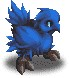
\includegraphics[width=0.23\columnwidth]{./art/chocobo/chocblue.jpg}}
{
	HP: & \hfill 15 & MP: & \hfill 25\\
	STR: & \hfill 0 & DEF: & \hfill 0 \\
	MAG: & \hfill 2 & RES: & \hfill 1 \\
	AGI: & \hfill 2 & STA: & \hfill 2 \\
}
{\accf{Beak}: 1d DMG \hfill \accf{Resilient:}\water}
{	
	\mspell{Water (Level 1)}{6}{0r}{Single}{4u}{You deal 2d water damage to the target.}{\accf{Level 1}\water}	
	\mspell{Accumulate (Level 3)}{3}{0r}{Single}{5u}{The target gains EnMAG for 3 rounds.}{\accf{Level 3}\enmag}	
	\mspell{Waterga (Level 6)}{14}{1r}{Single}{6u}{You deal 6d water damage to the target.}{\accf{Level 6}\water}	
	\mtech{Supersonic Wave (Level 9)}{18}{0r}{3u (front)}{Self}{All enemies in the target area suffer 4d damage and make a DC~8 check. Upon failure they suffer Silence for 3 rounds.}{\accf{Level 9}\silence}
	\mpassive{Choco Swim}{You can swim slowly through any river or sea without excessive current.}		
}
%
\clearpage
%
\ofmonster
{Green Chocobo}{1}{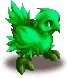
\includegraphics[width=0.23\columnwidth]{./art/chocobo/chocgreen.jpg}}
{
	HP: & \hfill 16 & MP: & \hfill 21\\
	STR: & \hfill 0 & DEF: & \hfill 1 \\
	MAG: & \hfill 1 & RES: & \hfill 1 \\
	AGI: & \hfill 2 & STA: & \hfill 2 \\
}
{\accf{Beak}: 1d DMG \hfill \accf{Immune:}\poison\blind\sleep}
{
	\mspell{Protect (Level 1)}{5}{0r}{Single}{5u}{The target gains EnDEF for 3 rounds.}{\accf{Level 1}\enndef}
	\mspell{Regen (Level 3)}{6}{0r}{Single}{5u}{The target gains regen for 3 rounds.}{\accf{Level 3}}	
	\mspell{Reflect (Level 6)}{10}{0r}{Single}{3u}{The target gains a shield that reflects the next spell that targets them back to its caster.}{\accf{Level 6}}	
	\mspell{Full-Life (Level 9)}{24}{1r}{Single}{3u}{Remove KO status from the target and fully restore his HP.}{\accf{Level 9}\ko}	
	\mpassive{Choco Mend}{Whenever you are not in combat, you can spend 10 minutes of time to cure an ally from any Status Effect except KO.}
}
%
\vfill
%
\ofmonster{White Chocobo}{1}{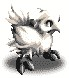
\includegraphics[width=0.23\columnwidth]{./art/chocobo/chocwhite.jpg}}
{
	HP: & \hfill 18 & MP: & \hfill 24\\
	STR: & \hfill 1 & DEF: & \hfill 0 \\
	MAG: & \hfill 1 & RES: & \hfill 1 \\
	AGI: & \hfill 2 & STA: & \hfill 3 \\
}
{\accf{Beak}: 1d DMG \hfill \accf{Resilient:}\holy}
{	
	\mspell{Haste (Level 1)}{8}{0r}{Single}{3u}{The target gains Haste for 3 rounds.}{\accf{Level 1}}
	\mspell{White Wind (Level 3)}{14}{0r}{4u (line)}{Self}{All allies in the target area regain an amount of HP equal to half of your current HP and are cured of all negative Status Effects except KO.}{\accf{Level 3}}
	\mspell{Recharge (Level 6)}{8}{1r}{3u}{Self}{All allies within the target area except you regain 3d MP.}{\accf{Level 6}}
	\mspell{Holy (Level 9)}{20}{2r}{Single}{7u}{You deal 6d+20 holy damage to the target.}{\accf{Level 9}\holy}
	\mpassive{Choco Sense}{You can sense the presence of hostile monsters in distance of up to 200u.}		
}
%
\vfill
%
\ofquote{"She’ll tell us when she’s ready, so just hold your Chocobos until then, ya?"}{Wakka}
%
\newpage
%
\ofmonster{Black Chocobo}{1}{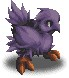
\includegraphics[width=0.23\columnwidth]{./art/chocobo/chocblack.jpg}}
{
	HP: & \hfill 19 & MP: & \hfill 23\\
	STR: & \hfill 1 & DEF: & \hfill 1 \\
	MAG: & \hfill 1 & RES: & \hfill 0 \\
	AGI: & \hfill 2 & STA: & \hfill 3 \\
}
{\accf{Beak}: 1d DMG \hfill \accf{Resilient:}\dark}
{
	\mspell{Gravity (Level 1)}{6}{0r}{Single}{3u}{The target suffers 2d damage and can only move half his usual distance on his next turn. 
	}{\accf{Level 1}}
	\mspell{Petrify (Level 3)}{7}{1r}{Single}{5u}{The target makes a DC 8 and suffers Immobile for 3 rounds upon failure.}{\accf{Level 3}\immobile}
	\mspell{Imperil (Level 6)}{10}{1r}{Single}{5u}{The target suffers DeDEF and DeRES for 3 rounds}{\accf{Level 6}\dedef \deres}	
	\mspell{Ultima (Level 9)}{25}{2r}{2u}{7u}{Deal 6d+35 dark damage to all enemies in the target area.}{\accf{Level 9}\dark}
	\mpassive{Choco Fly}{You can fly up to 50u above the ground.}		
}
%
\vfill
%
\ofmonster{Golden Chocobo}{1}{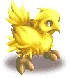
\includegraphics[width=0.23\columnwidth]{./art/chocobo/chocgold.jpg}}
{
	HP: & \hfill 25 & MP: & \hfill 35\\
	STR: & \hfill 1 & DEF: & \hfill 1 \\
	MAG: & \hfill 1 & RES: & \hfill 1 \\
	AGI: & \hfill 3 & STA: & \hfill 3 \\
}
{\accf{Beak}: 2d DMG \hfill \accf{All-Immune}}
{
	\mtech{Shine (Level 1)}{5}{0r}{3u}{Self}{All enemies in the target area perform a DC 7 check and suffer Blind for 2 rounds upon failure.}{\accf{Level 1}\blind}
	\mtech{Good Breath (Level 3)}{8}{0r}{3u (front)}{Self}{Remove all Status Effects except KO from all allies in the target area.}{\accf{Level 3}}	
	\mspell{Diaga (Level 5)}{14}{1r}{Single}{6u}{You deal 6d holy damage to the target.}{\accf{Level 5}\fire}
	\mspell{Curaja (Level 7)}{20}{2r}{3u}{5u}{All allies in the target area regain 6d+15 HP.}{\accf{Level 7}}	
	\mtech{Choco Meteor (Level 8)}{27}{2r}{3u}{10u}{Everyone in the target area suffers 6d+40 damage.}{\accf{Level 8}}	
	\mtech{Final Phoenix (Level 10)}{30}{2r}{3u}{Self}{Remove KO from all allies in the target area and fully restore their HP.}{\accf{Level 10}}	
	\mpassive{Choco Sense}{You can sense the presence of hostile monsters in distance of up to 200u.}		
	\mpassive{Choco Fly}{You can fly up to 50u above the ground.}	
}
%
\clearpage